\begin{scanpage}{0121}{104}
\noindent\begin{minipage}[t]{.34\linewidth}\vspace{0pt}\centering
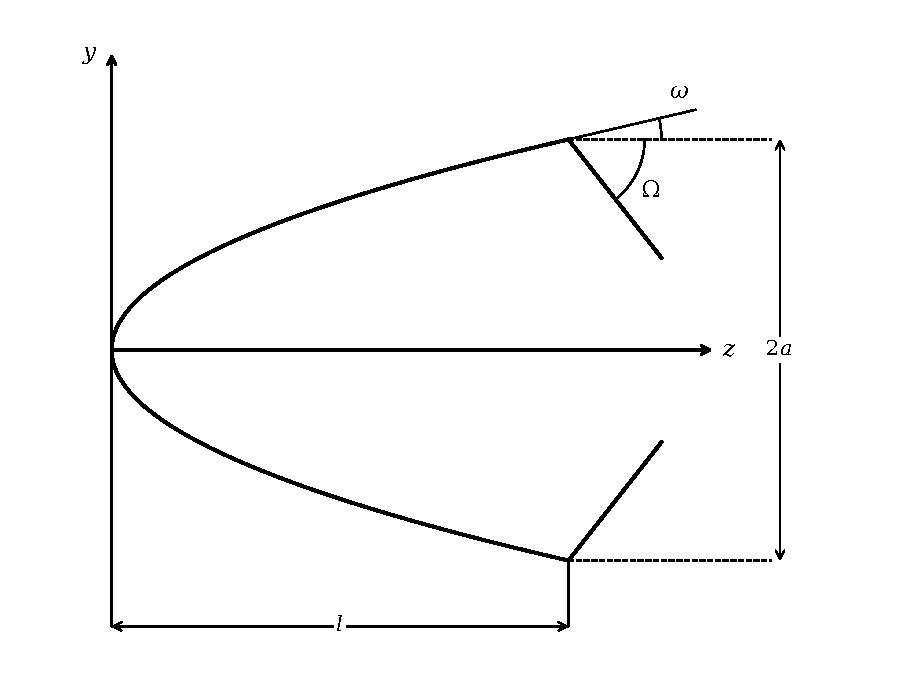
\includegraphics[width=\linewidth]{images/recreated/b-0121-fig36.pdf}

Figure 36. Diffraction of a plane wave by a paraboloid of rotation.
\end{minipage}\hfill\begin{minipage}[t]{.62\linewidth}\vspace{0pt}
The field from the nonuniform part of the current caused by the discontinuity of the paraboloid's surface is determined by Equation (17.03). The field from the nonuniform part of the current which is caused by the smooth curve of the paraboloid's surface equals zero in the case of symmetric radiation [45]. Therefore, summing (18.02) and (17.03) we find the expression for the resulting fringing field:
\end{minipage}
\[\left.\begin{aligned}E_x=-H_y&=-\frac{aE_{0x}}2\left(\operatorname{tg}\omega+\frac{\frac2n\sin\frac\pi n}{\cos\frac\pi n-\cos\frac{2\omega}n}e^{2ikl}\right)\frac{e^{ikR}}R,\\E_y=H_x&=0\\&\left(n=1+\frac{\omega+\Omega}\pi\right).
\end{aligned}\right\}\tag{18.03}\]
Consequently, the effective scattering area of the paraboloid will be determined by the relationship
\[\sigma=\pi a^2\left|\operatorname{tg}\omega+\frac{\frac2n\sin\frac\pi n}{\cos\frac\pi n-\cos\frac{2\omega}n}e^{2ikl}\right|^2,\tag{18.04}\]
which, when the paraboloid is deformed into a disk $(\omega\to\frac\pi2,\ l\to0,\ \Omega=\mathrm{const})$, is transformed to the form
\[\sigma=\pi a^2\left|ika+\frac1n\operatorname{ctg}\frac\pi n\right|^2.\tag{18.05}\]
Comparing Expression (18.04) with the equation
\[\sigma^0=\pi a^2\operatorname{tg}^2\omega\,|1-e^{2ikl}|^2,\tag{18.06}\]
which physical optics gives for the effective scattering area, we see that they differ significantly from one another. First of all, the oscillating character of the function $\sigma^0$ draws our attention:
\end{scanpage}
